\section{Results}\label{sec:results}

\subsection{Older Danes living alone}

Table~\ref{tab:dkold} reports the test for Danes aged 65 and over who live alone. For the group as a whole the evidence against unimodality grows with the sample: the $p$-value is at or near one in 2004 and 2007, $0.105$ in 2010, and $0.035$, $0.015$ and $0.005$ in 2013, 2016 and 2019. In each of the three rejecting waves the valley is one or two cells wide and lies between 132{,}500 and 152{,}500 kroner, and the upper mode is 30{,}000 to 40{,}000 kroner above the lower one. The lower mode moves with the pension. Measured by the centre of its cell it is at 125{,}000, 135{,}000 and 140{,}000 kroner in the three rejecting waves, 0.88, 0.90 and 0.88 of the gross full pension of Table~\ref{tab:floors}. In 2010, where the test falls just short of rejecting ($p=0.105$), the maximising split puts the lower mode at 110{,}000 kroner, 0.83 of the pension.

\begin{table}[t]
\centering\small
\caption{Tests of unimodality for the disposable income of Danes aged 65 and over living alone. Cells of 5{,}000 kroner between the 5th and 95th percentiles of the group; 199 bootstrap draws. $p$: bootstrap $p$-value; modes: centres of the cells containing the two modes, in thousands of kroner, reported when $p\le0.10$. Transfer-reliant: public pensions and benefits at least 90 per cent of income.}\label{tab:dkold}
\begin{tabular}{lrrcrrcrrr}
\toprule
 & & \multicolumn{2}{c}{All 65+} & \multicolumn{3}{c}{Transfer-reliant} & Other & \multicolumn{2}{c}{By age: $p$}\\
\cmidrule(lr){3-4}\cmidrule(lr){5-7}\cmidrule(lr){8-8}\cmidrule(lr){9-10}
Year & $n$ & $p$ & modes & share & $p$ & modes & $p$ & 65--74 & 75+\\
\midrule
2004 & 11{,}855 & 1.000 & & 0.58 & 0.025 & 90, 120 & 1.000 & 1.000 & 0.005\\
2007 & 11{,}865 & 1.000 & & 0.53 & 0.005 & 95, 130 & 0.995 & 1.000 & 0.225\\
2010 & 12{,}682 & 0.105 & & 0.53 & 0.005 & 110, 150 & 1.000 & 1.000 & 0.005\\
2013 & 13{,}272 & 0.035 & 125, 155 & 0.51 & 0.005 & 120, 160 & 0.650 & 1.000 & 0.005\\
2016 & 42{,}971 & 0.015 & 135, 170 & 0.60 & 0.005 & 135, 170 & 1.000 & 0.955 & 0.005\\
2019 & 45{,}496 & 0.005 & 140, 180 & 0.59 & 0.005 & 135, 180 & 0.180 & 1.000 & 0.005\\
\bottomrule
\end{tabular}
\end{table}

The source of the second mode becomes visible when the group is split by where its income comes from. Between 51 and 60 per cent of older Danes living alone receive at least nine tenths of their income from public pensions and benefits. Among them the test rejects in every wave, with $p$-values of $0.025$ in 2004 and $0.005$, the smallest attainable with 199 draws, in every later wave, although the transfer-reliant group numbers only 6{,}300 to 6{,}900 people in the four earlier waves. Among older people with substantial occupational or private pensions, earnings or capital income there is no evidence against unimodality in any wave. The same is true of people aged 65 to 74, while for those aged 75 and over, of whom 55 to 67 per cent are transfer-reliant against 46 to 54 per cent of the younger group, the test rejects in five of the six waves. The bimodality is thus a property of the transfer-reliant, and it shows in the whole group only to the extent that they dominate it.

The result does not depend on the 90 per cent threshold. With a threshold of 95 per cent the test rejects at $p=0.005$ in every wave from 2007 and gives $p=0.13$ in 2004; with 80 per cent, which admits more people with small occupational pensions, it rejects at $p=0.005$ in every wave from 2010 but not in 2004 and 2007. A second refinement matters more for what follows. In Denmark the LIS item for public contributory pensions contains the statutory funded supplement ATP, which is usually small, and the pensions of former civil servants, which can be large: in 2016 and 2019 a tenth of the transfer-reliant group has public contributory pensions of more than 140{,}000 kroner. Excluding everyone whose public contributory pensions exceed a tenth of income removes the former civil servants together with those whose ATP pension is large. It leaves 43 to 54 per cent of the older population, among whom the test rejects at $p=0.005$ in every wave, with modes at 90 and 120 thousand kroner in 2004 rising to 135 and 180 thousand in 2019. At a cell width of 10{,}000 kroner the test rejects for this group in every wave ($p=0.03$ in 2004, $0.01$ in 2007 and $0.005$ thereafter), and for all people aged 65 and over in 2016 ($p=0.03$) and 2019 ($0.005$). Shifting the cell grid by half a cell, so that the cells are centred at odd multiples of 2{,}500 kroner, leaves these rejections at $p=0.005$ in 2016 and 2019 and moves the valley by at most 5{,}000 kroner. This refined group is the one on which the rest of the analysis rests, and its test is the paper's primary test. Many other tests are reported, but for the primary one a Holm correction across the six waves still gives adjusted $p$-values of at most $0.03$.

\subsection{Two floors}

\begin{figure}[t]
\centering
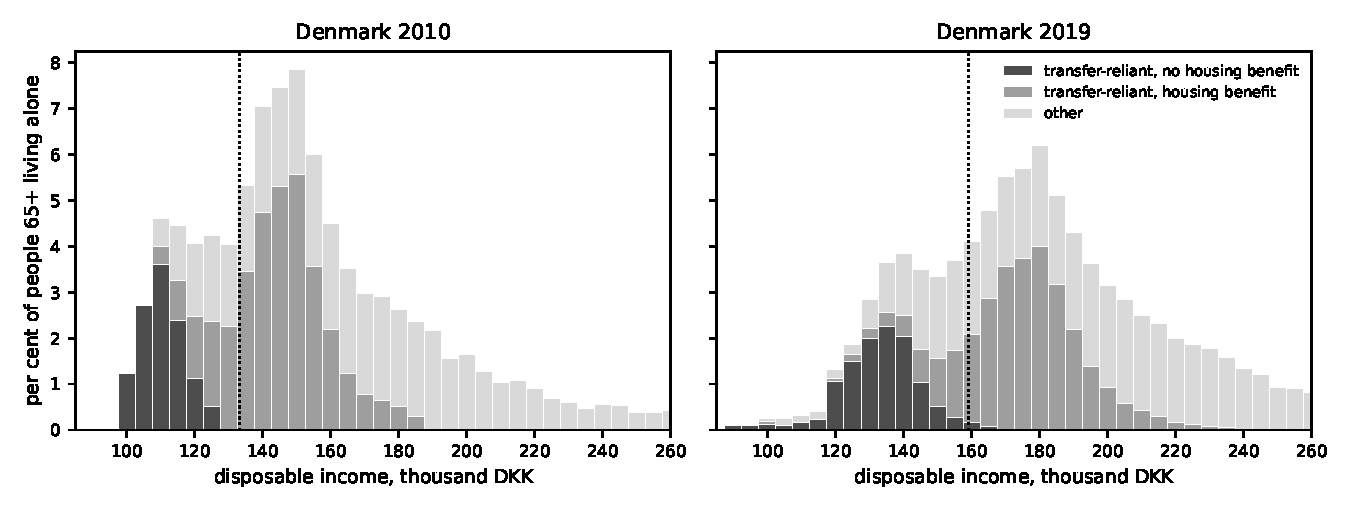
\includegraphics[width=\textwidth]{fig/dk_stack.pdf}
\caption{Disposable income of Danes aged 65 and over living alone, 2010 and 2019, in cells of 5{,}000 kroner, as a percentage of the group. The bars are stacked by source of income: transfer-reliant (public pensions and benefits at least 90 per cent of income, public contributory pensions at most 10 per cent) without and with the pensioners' housing benefit, and everyone else. Cells with fewer than 30 observations in a component are suppressed and shown as zero. Dotted line: gross annual folkepension for a single person at the full rate (Table~\ref{tab:floors}).}\label{fig:stack}
\end{figure}

Figure~\ref{fig:stack} shows the decomposition for 2010 and 2019. The transfer-reliant without the housing benefit form a narrow peak 15 to 20 per cent below the gross full pension, the transfer-reliant with the benefit a second peak 40{,}000 to 45{,}000 kroner higher, and everyone else a broad hump that extends far to the right. The dip between the two peaks is visible in the total for 2019; in 2010 it is filled in by the broad hump, which is why the whole group shows a second mode only in the later waves.

Table~\ref{tab:hb} splits this refined transfer-reliant group by whether they receive the pensioners' housing benefit. Seventy-one to 76 per cent do. Among recipients the test does not reject in any wave, and among non-recipients it does not reject in any wave; in every case the $p$-value is one. Each group has a single mode, and the two modes are those of the pooled group. The lower one is the net pension. In the LIS data the most common folkepension payment among the transfer-reliant from 2010 onwards is the full pension plus the ældrecheck (143{,}972 kroner in 2010, 157{,}884 in 2013, 166{,}144 in 2016 and 176{,}600 in 2019), and the median disposable income of non-recipients is a stable 75 to 77 per cent of it: what remains of that sum after income tax, with little else added or taken away. The groups are also tight: the interquartile range of disposable income is 8{,}000 to 15{,}000 kroner among non-recipients and 15{,}000 to 21{,}000 kroner among recipients, less than the distance between their medians in every wave. The distance between the medians of the two groups is 26{,}000 kroner in 2004, rising to 42{,}000 in 2019, and it is close to the median benefit received, which rises from 28{,}000 to 40{,}000 kroner over the same period. The benefit in the data behaves as the statute says it should. Among recipients in the refined group, 15.7 per cent in 2016 and 14.3 per cent in 2019 receive exactly the statutory annual maximum of 45{,}480 and 48{,}540 kroner, and the 75th percentile of the benefit equals the maximum to the krone in both years. The LIS item exceeds the maximum for another 14 to 17 per cent of recipients, which suggests that it also contains some housing support other than the pensioners' benefit.

\begin{table}[t]
\centering\small
\caption{Transfer-reliant Danes aged 65 and over living alone, excluding those whose public contributory pensions exceed a tenth of income, split by receipt of the pensioners' housing benefit. Share: of all people aged 65 and over living alone; HB: share receiving the housing benefit; medians in thousands of kroner; $p$: bootstrap $p$-values as in Table~\ref{tab:dkold}; owners: share of owner-occupiers among the non-recipients of the (unrefined) transfer-reliant group.}\label{tab:hb}
\begin{tabular}{lrrrrrrrrr}
\toprule
 & & & \multicolumn{3}{c}{Median} & \multicolumn{3}{c}{$p$} & \\
\cmidrule(lr){4-6}\cmidrule(lr){7-9}
Year & Share & HB & benefit & dhi, HB & dhi, no HB & pooled & HB & no HB & owners\\
\midrule
2004 & 0.54 & 0.71 & 28.0 & 117.8 & 91.7 & 0.005 & 1.000 & 1.000 & 0.72\\
2007 & 0.50 & 0.76 & 29.8 & 127.2 & 95.9 & 0.005 & 1.000 & 1.000 & \\
2010 & 0.49 & 0.74 & 32.8 & 145.0 & 110.3 & 0.005 & 1.000 & 1.000 & 0.73\\
2013 & 0.47 & 0.74 & 36.1 & 156.7 & 118.4 & 0.005 & 1.000 & 1.000 & \\
2016 & 0.44 & 0.73 & 39.0 & 165.6 & 126.5 & 0.005 & 1.000 & 1.000 & 0.67\\
2019 & 0.43 & 0.71 & 40.4 & 175.5 & 133.7 & 0.005 & 1.000 & 1.000 & 0.65\\
\bottomrule
\end{tabular}
\end{table}

Who are the two groups? In the transfer-reliant group before the refinement, 99.8 to 99.9 per cent of recipients of the housing benefit rent their home, and 65 to 73 per cent of non-recipients own it. The lower mode is therefore, for the most part, older owner-occupiers living on the folkepension, and the upper mode older renters living on the folkepension and the housing benefit. The difference between them is the benefit: the median transfer-reliant renter has a disposable income 22{,}000 to 34{,}000 kroner higher than the median transfer-reliant owner, and the difference is the housing benefit that pays part of her rent.

\subsection{Removing the housing benefit}\label{sec:cf}

If the second mode is the housing benefit, subtracting the benefit from each person's disposable income should remove it. Table~\ref{tab:cf} reports the test before and after the subtraction, for the whole group aged 65 and over and for the refined transfer-reliant group. Before, the test rejects for the transfer-reliant group in every wave and for the whole group from 2013; after, the smallest $p$-value in either group in any wave is $0.99$. The subtraction leaves the non-recipients where they were and moves each recipient down by her benefit; that this is enough to remove the valley means that, net of the benefit, recipients and non-recipients have the same distribution to within the resolution of the test. The quartiles show it directly. In 2019 the quartiles of disposable income less the benefit among recipients are 129{,}400, 135{,}000 and 141{,}000 kroner, and the quartiles of disposable income among non-recipients are 125{,}700, 133{,}700 and 140{,}600 kroner; in 2004 they are 87{,}000, 89{,}400 and 92{,}300 against 88{,}000, 91{,}700 and 96{,}200. Net of the benefit, pensioners who receive it and pensioners who do not have almost the same distribution of income.

\begin{table}[t]
\centering\small
\caption{Tests of unimodality for disposable income (dhi) and for disposable income less the housing benefit (dhi$-$hb), Danes aged 65 and over living alone and the refined transfer-reliant group of Table~\ref{tab:hb}. Cells of 5{,}000 kroner, lowest 5 per cent trimmed, 199 bootstrap draws. Valley and modes in thousands of kroner, reported when $p\le0.10$.}\label{tab:cf}
\begin{tabular}{lrlrrlr}
\toprule
 & \multicolumn{3}{c}{All 65+} & \multicolumn{3}{c}{Transfer-reliant}\\
\cmidrule(lr){2-4}\cmidrule(lr){5-7}
Year & $p$, dhi & valley; modes & $p$, dhi$-$hb & $p$, dhi & valley; modes & $p$, dhi$-$hb\\
\midrule
2004 & 1.000 & & 0.990 & 0.005 & 97.5--107.5; 90, 120 & 1.000\\
2010 & 0.105 & & 1.000 & 0.005 & 117.5--132.5; 110, 150 & 1.000\\
2013 & 0.035 & 132.5--137.5; 125, 155 & 1.000 & 0.005 & 127.5--142.5; 120, 160 & 1.000\\
2016 & 0.015 & 137.5--147.5; 135, 170 & 1.000 & 0.005 & 137.5--152.5; 130, 170 & 1.000\\
2019 & 0.005 & 142.5--152.5; 140, 180 & 1.000 & 0.005 & 142.5--157.5; 135, 180 & 1.000\\
\bottomrule
\end{tabular}
\end{table}


\subsection{Norway}

Table~\ref{tab:no} reports the same analysis for Norwegians aged 67 and over living alone. There is no evidence against unimodality in any register wave, at either cell width. The minimum pension is visible in the data: the tenth percentile of the disposable income of transfer-reliant older Norwegians is within seven per cent of the minimum pension in every wave up to 2019 and coincides with it in 2016 (in 2022 it is 15 per cent below it), and gross and disposable income of this group are almost the same, as the tax rules imply. But the transfer-reliant are only four to seven per cent of the older population living alone, against half in Denmark, and their incomes form the lower shoulder of a single mode rather than a mode of their own. The Danish data show that this share is decisive. Keeping all older Danes who are not transfer-reliant and a random subsample of the transfer-reliant, so that they make up 6 or 30 per cent of the group rather than 59 or 60, the test did not reject in any of eight subsamples at either share in 2016 or 2019. Nor is the Norwegian housing allowance the difference: 54 and 68 per cent of transfer-reliant older Norwegians received it in 2016 and 2019, but the median amount, 17{,}500 and 18{,}500 kroner, is less than a tenth of their median disposable income, against almost a quarter of the median disposable income of Danish recipients, and tenure does not split them: the median disposable income of transfer-reliant owners is only 5{,}000 to 8{,}500 kroner above that of renters.

\begin{table}[t]
\centering\small
\caption{Norwegians aged 67 and over living alone. Cells of 5{,}000 and 10{,}000 kroner between the 5th and 95th percentiles; 199 bootstrap draws. Floor: calendar-year average minimum pension for a single person (Table~\ref{tab:floors}; 2022 from \citealp{NOMeld2022}); reliant: transfer-reliant share; q10: tenth percentile of disposable income among the transfer-reliant, in thousands of kroner.}\label{tab:no}
\begin{tabular}{lrrrrrrr}
\toprule
 & & & & & \multicolumn{3}{c}{$p$}\\
\cmidrule(lr){6-8}
Year & $n$ & Floor & Reliant & q10 & all, $w=5$k & all, $w=10$k & other\\
\midrule
2007 & 23{,}505 & 117.5 & 0.065 & 125.7 & 1.000 & 1.000 & 1.000\\
2010 & 23{,}920 & 148.7 & 0.067 & 157.9 & 1.000 & 1.000 & 1.000\\
2013 & 24{,}957 & 166.2 & 0.053 & 173.0 & 1.000 & 0.435 & 1.000\\
2016 & 26{,}504 & 179.7 & 0.062 & 179.7 & 0.750 & 0.130 & 0.990\\
2019 & 28{,}314 & 198.6 & 0.041 & 192.5 & 0.870 & 0.675 & 1.000\\
2022 & 30{,}782 & 230.2 & 0.056 & 194.7 & 0.970 & 1.000 & 0.610\\
\bottomrule
\end{tabular}
\end{table}

\subsection{Other countries}\label{sec:countries}

This subsection shows that the two-floor structure is not a Danish peculiarity: it appears where the conditions it requires are met, and there too removing the housing allowance removes it.

\paragraph{Conditions.} The Danish and Norwegian results point to three conditions. (C1) A large share of the group lives on a statutory floor, so that its disposable income is fixed by statute. (C2) A second transfer is paid to a substantial part of that group but not to all of it. (C3) The second transfer separates the two parts: the distance between their medians is large relative to the spread of income within each. (C2) and (C3) decide whether the income of those on the floor is bimodal; (C1) decides whether that bimodality is visible in the group as a whole, as the Danish subsampling exercise of the previous subsection shows. In Denmark 71 to 76 per cent of the refined transfer-reliant group receive the housing benefit, and the distance between the medians of recipients and non-recipients is 2.8 to 3.5 times the interquartile range of non-recipients and 1.7 to 2.0 times that of recipients. Norway fails (C1), and (C3) as well.

(C2) can be quantified with the Danish data. Keep all non-recipients in the refined group of 2019 and a random subsample of recipients, so that recipients are 22 per cent of the group instead of 71. The test then rejects at the 5 per cent level in all ten subsamples, of about 7{,}300 people each, but in only two of ten when the subsample is cut to 1{,}000 people. With recipients at 10 per cent it rejects in none of ten subsamples at either size. A second transfer received by a fifth of the group can split it, but only in a large sample; one received by a tenth does not.

\paragraph{Data and design.} Most other LIS files are survey samples with a few hundred to a few thousand older people living alone in each wave, too few for the test (Appendix~\ref{app:sefi}). I therefore pool all waves from 2010 to 2021 for eight countries that record a housing allowance in LIS (item hi46) and have several thousand older people living alone across the waves: the Netherlands, the United Kingdom, Australia, Ireland, the United States, France, Sweden and Germany. Other LIS countries with the item were not examined. Pooling needs a common scale, because benefit rates and incomes change from wave to wave. In each wave income is expressed as a percentage of the median disposable income of transfer-reliant non-recipients of the allowance, the analogue of the Danish lower floor, so that this median is 100 in every wave. The group is the transfer-reliant group as defined above. The refinement that excludes public contributory pensions cannot be used outside Denmark, because in the United Kingdom, Ireland, the United States and Germany the main public old-age pension is itself recorded as contributory. Denmark is run through the same procedure, with its 2016 and 2019 waves, as a control. Table~\ref{tab:pool} reports the results. Because each wave is placed so that its non-recipients sit at 100, pooling cannot move a mode that no single wave has; it could, however, blur a second mode whose position varies from wave to wave, or produce one from waves whose single modes lie at different points. Two checks address this. Where the waves are large enough, the test is also run wave by wave; and for Denmark, the Netherlands, the United Kingdom, Australia and Ireland the pooled test is repeated with incomes divided by the median of all transfer-reliant people in the wave instead of non-recipients.

\begin{table}[t]
\centering\footnotesize
\caption{Transfer-reliant people aged 65 and over living alone (public pensions and benefits at least 90 per cent of income), all LIS waves 2010--2021 pooled. In each wave income is divided by the median disposable income of transfer-reliant non-recipients of a housing allowance and multiplied by 100, so that this median is 100 in every wave; household weights are normalised to average one within each wave. $n$: pooled number of transfer-reliant; share: of all aged 65 and over living alone; HB: share of the transfer-reliant receiving a housing allowance (LIS item hi46); benefit and gap: range over waves of the median allowance of recipients and of the difference between the median incomes of recipients and non-recipients, both on the same scale. $p$: bootstrap $p$-values of the test of unimodality, lowest 5 per cent trimmed, 199 draws, with cells of 2 and 4 points of the scale; less HB: income less the allowance, cells of 2; HB, no HB: recipients and non-recipients separately, cells of 2, tested when the pooled test rejects at the 10 per cent level. Denmark: waves 2016 and 2019 only, as a control; its no-HB and less-HB rejections come from former civil servants, and in the refined group of Table~\ref{tab:hb}, pooled in the same way, the $p$-values for less HB, HB and no HB are 1.000, 0.650 and 0.325.}\label{tab:pool}
\setlength{\tabcolsep}{3pt}
\begin{tabular}{lrrrrrrrrrrr}
\toprule
 & & & & & & & \multicolumn{5}{c}{$p$}\\
\cmidrule(lr){8-12}
Country & Waves & $n$ & Share & HB & Benefit & Gap & 2 & 4 & less HB & HB & no HB\\
\midrule
Denmark & 2 & 52{,}336 & 0.59 & 0.61 & 27--28 & 25 & 0.005 & 0.005 & 0.005 & 0.975 & 0.005\\
Netherlands & 12 & 3{,}315 & 0.16 & 0.65 & 19--23 & 18--25 & 0.010 & 0.005 & 0.195 & 1.000 & 0.005\\
United Kingdom & 12 & 13{,}185 & 0.38 & 0.66 & 41--47 & 47--55 & 0.005 & 0.005 & 0.315 & 0.005 & 0.065\\
Australia & 5 & 5{,}332 & 0.56 & 0.17 & 13--15 & 13--23 & 0.005 & 0.250 & 0.325 & 0.665 & 0.050\\
Ireland & 12 & 7{,}432 & 0.82 & 0.88 & 6--11 & $-40$ to 9 & 0.005 & 0.005 & 0.005 & 0.005 & 0.995\\
United States & 12 & 38{,}972 & 0.51 & 0.16 & 16--21 & $-7$ to 2 & 0.055 & 0.005 & 0.165 & 1.000 & 0.070\\
France & 12 & 8{,}964 & 0.10 & 0.87 & 10--22 & 3--41 & 0.190 & 0.450 & 0.150 & & \\
France 2010--14 & 5 & 3{,}939 & 0.10 & 0.89 & 18--22 & 38--41 & 0.005 & 0.005 & 0.425 & & \\
Sweden & 12 & 2{,}640 & 0.24 & 0.63 & 22--30 & 0--17 & 1.000 & 0.855 & 0.125 & & \\
Germany & 12 & 10{,}923 & 0.66 & 0.04 & 4--8 & $-45$ to $-33$ & 0.685 & 0.645 & 0.925 & & \\
\bottomrule
\end{tabular}
\end{table}


\paragraph{Replications.} The procedure reproduces the Danish result: the pooled Danish transfer-reliant group is bimodal ($p=0.005$) with modes at 96 and 126 on the scale, as is each of the two waves and the pool on the alternative scale, and in the refined group recipients, non-recipients and income less the benefit are each unimodal.

The Netherlands has the Danish structure on a smaller scale. The flat-rate state pension (AOW) is the floor for 16 per cent of older people living alone; 65 per cent of them receive the housing allowance (huurtoeslag), whose median is 19 to 23 per cent of the floor. The pooled test rejects ($p=0.010$ with cells of 2 points, $0.005$ with cells of 4), with modes at 100 and 124: the floor, and the floor plus the allowance. Recipients alone are unimodal ($p=1$), and subtracting the allowance from income removes the valley ($p=0.195$). On the alternative scale the test also rejects ($p=0.005$). The Dutch waves have 120 to 480 transfer-reliant people each, too few to test one at a time, but in every wave the cells of the pooled valley hold less mass than the cells of equal width around the upper mode. Non-recipients show a further mode at 60 per cent of the floor. This is consistent with the rule that the AOW accrues at 2 per cent for each year of residence, so that people who spent part of their working lives abroad receive a partial pension; I do not pursue it.

In the United Kingdom the transfer-reliant are 38 per cent of older people living alone, and two thirds of them receive support with housing costs, which LIS records in hi46 and which comprises Housing Benefit and council-tax support. The pooled distribution is bimodal ($p=0.005$ at both cell widths), with modes at 102 and 148, and it is unimodal once the housing support is subtracted ($p=0.315$). On the alternative scale the test rejects as well ($p=0.005$). Wave by wave, with 1{,}000 to 1{,}400 people each (524 in 2020), it rejects at the 5 per cent level in 2011, 2016 and 2021, and in these waves the modes lie at 100 to 104 and 136 to 152, where the pooled modes are. Unlike the Danish recipients, the British recipients are themselves bimodal. Housing Benefit pays a share of the actual rent, not a sum bounded by a low maximum, and council-tax support on its own is small, so recipients do not share one amount. When recipients are split by the size of the payment, measured here against the median income of all transfer-reliant in the wave, recipients of more than 15 per cent of that median are unimodal ($p=0.99$), and without the fifth of the group who receive smaller amounts the distribution is only weakly bimodal ($p=0.07$). The British structure is thus the floor, on which non-recipients and recipients of council-tax support alone both stand, and the floor plus Housing Benefit.

France shows the structure appearing and disappearing with (C3). Ten per cent of older people living alone are transfer-reliant, and nine in ten of them receive a housing allowance. From 2010 to 2014 the median income of recipients was 38 to 41 per cent above that of non-recipients, and the pooled distribution of these five waves is bimodal ($p=0.005$ at both cell widths) with modes at 100 and 132; subtracting the allowance removes the valley ($p=0.425$). The gap then shrank, to 3 per cent in 2021, and with all twelve waves pooled the second mode is smeared out ($p=0.19$).

Australia is the marginal case that (C2) predicts, and the evidence there is marginal too. Fifty-six per cent of older people living alone live on the Age Pension, but only 17 per cent of them receive Rent Assistance, which amounts to 13 to 15 per cent of the floor. With cells of 2 points the pooled test rejects ($p=0.005$), with modes at 100 and 114, and subtracting Rent Assistance removes the valley ($p=0.325$). But with cells of 4 points, which make the gap between the modes three cells wide, it does not reject ($p=0.25$); on the alternative scale it gives $p=0.065$; and no single wave rejects at the 5 per cent level. Non-recipients alone give $p=0.05$, with a shallow dip just below the floor (modes at 90 and 100); whatever produces it, it is not Rent Assistance, and it lies below the valley at 109 to 113 that the pooled test finds. The Danish experiment says that a recipient share of this size is detectable only in large samples, so the Australian result is what the conditions predict, but it is not a replication.

\paragraph{Countries without the structure.} In Germany only 4 per cent of the transfer-reliant receive a housing allowance, and recipients are poorer, not richer, than non-recipients. (C2) fails, and the test does not reject. In Sweden recipients of the housing supplement are barely richer than non-recipients: the gap between the medians is 0 to 17 points of the scale, while the interquartile range among non-recipients is 26 to 36 points. (C3) fails, and the test does not reject.  In the United States housing assistance reaches 16 per cent of the transfer-reliant and does not separate them from the rest (the gap is $-7$ to 2 points), and non-recipients are widely spread (interquartile range 57 to 72 points), so there is no floor for the allowance to lift anyone above: (C3) fails. With cells of 4 points the test finds a shallow second mode 8 points above the first ($p=0.005$, excess mass 0.004 against 0.026 in Denmark). It is unrelated to housing assistance, since recipients alone give $p=1$; the two cell widths locate the dip in different places, and at this sample size the test is slightly liberal (Section~\ref{sec:data}). I read it as noise. In Ireland 88 per cent of the transfer-reliant receive a housing-related payment, and it is small (6 to 11 points), so (C3) fails. The Irish pooled test rejects, but the rejection survives the subtraction of the payment ($p=0.005$), and its location depends on the scale: when incomes are divided by the median of all transfer-reliant rather than of non-recipients, the valley is a single cell 2 points wide, with the two modes in the adjacent cells at 96 and 100. Whatever produces it, it is not the housing payment.

The conditions thus sort the countries. Where a housing allowance is paid to a substantial part of a group living on a flat floor and lifts them clearly above it (Denmark, the Netherlands, the United Kingdom, and France until 2014), the income of the group has two modes, and subtracting the allowance removes the second. Where the recipient share is small (Australia) the evidence is weak, as the Danish experiment says it must be. Where a condition fails (Norway, Sweden, Germany, the United States, Ireland, and France after the gap closed), no second mode is due to the allowance.

\subsection{Working-age people living alone}

People aged 30 to 64 living alone are the natural comparison: few of them live on a flat-rate transfer. With the lowest five per cent trimmed, the $p$-values are between $0.06$ and one in every wave, and with the lowest ten per cent trimmed between $0.14$ and one. There is no evidence of a second mode among working-age singles. The same is true in Norway in every register wave but the last, 2022, where the test rejects with a shallow valley between 297{,}500 and 352{,}500 kroner, far above any statutory amount; I do not pursue it here.
